\documentclass{article}
\usepackage{float,amsmath}
\usepackage{graphicx}
\usepackage{color}
\usepackage[a4paper,margin=2cm]{geometry}
\usepackage{hyperref}

%\setlength{\textwidth}{6.5in}

\begin{document}

\author{David DeBoer}
\title{HERA Dimensions} 
\maketitle

\section{Hub and Support Spar}
\begin{figure}[H]
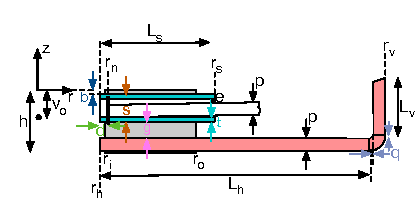
\includegraphics[width=0.8\textwidth]{hubdims.pdf}
\centering
\vspace{-.15in}
\caption{General dimensions of hub and support spar (colored light red).}
\label{fig:hubdims}
\end{figure}

\begin{tabular}{l l}
$h$          & height of hub \\
$v_o$      & distance of vertex from top of hub \\
$b$          & distance between top of hub and top of sleeve \\
$L_s$      & length of sleeve \\
$s$          & outer diameter of sleeve \\
$t$           & wall thickness of sleeve \\
$g$          & distance between bottom of sleeve and top of horizontal support spar \\
$d$          & distance between nail and the inner edge of the sleeve \\
$q$          & distance between 90$^o$ coupler spar and and orthogonal edge \\
$e$          & spacer-gap at outer edge of sleeve \\
$h_v$      & distance between top of horizontal support spar and lower edge of vertical support spar \\
$r_i$        & radial distance to inner edge of hub  \\
$r_o$       & radial distance to outer edge of hub  \\
$r_n$       & radial distance to nail  \\
$r_s$       & radial distance to end of sleeve  \\
$r_h$       & radial distance to inner edge of horizontal support \\
$L_h$      & length of horizontal support spar \\
$L_v$      & long length of vertical support spar \\
$F$          & focal length of parabola \\
$z$          & height z with 0 at top of hub \\
$r$           & radial distance with 0 at center of hub\\
$\theta(r)$& = $\tan^{-1}(r/2F)$
\end{tabular}
%\vspace{.in}

The hub is a concrete ``donut'' made up of two concentric rings with holes cut in to allow PVC spars to be positioned.  There are two sets of spar holes, each of which have twelve equi-spaced holes in the inner and outer rings.  There is another small hole $v_o$ from the top of the inner ring to accommodate a piece of rebar.  The bottom holes have diameter $p$ and the top holes have diameter $s$.  The bottom holes are centered $b+s+g+p/2$ from the top of the hub and the top holes are centered $b+s/2$ from the top.  The hub height is $h$.

\subsection{Sleeve and Vertex Offset}
To get the offset between the top of the hub and the vertex, we need to set the sleeve in one of two ways:

\vspace{.3in}
\noindent
{\bf 1:}  Given $s, t$, design the sleeve to the correct length $L_s$ (so $e=0$).
Matching the angle at the exit from the sleeve to the proper parabolic angle (see Sec. \ref{sec:derive}):
\begin{equation}
r_s = \frac{r_n + \sqrt{r_n^2 + 8(s - 2t - p)F}}{2}
\label{eq:sleeveExitAngle}
\end{equation}
Then $L_s = r_s - r_n + d$.

\vspace{0.2in}
\noindent
{\bf 2:}  Make a sleeve ($s, t, L_s$) then include a spacer $e$.  Then $r_s = L_s + r_n - d$ and 
\begin{equation}
e = (s - 2t - p) + \frac{r_s(r_s - r_n)}{2F}
\label{eq:spacer}
\end{equation}
\noindent
Then
\begin{equation}
v_o = b + t + e + \frac{r_s^2}{4F}
\end{equation}

\subsection{Parabolic Offsets from Top of Hub}
\noindent
Height from the top of the hub surface to the top of the spar ($z_t$) at radius $r$:
\begin{equation}
z_t(r) = \left(\frac{r^2}{4F}\right) - v_o
\end{equation}

\noindent
Height from the top of the hub surface to the bottom of the spar ($z_b$) at radius $r$:
\begin{equation}
z_b(r) = z_t - \left(\frac{p}{\cos\theta(r)}\right) = \left(\frac{r^2}{4F}\right) - \left(\frac{p}{\cos\theta(r)}\right) - v_o \approx \left[\frac{r^2}{4F(1+p/2F)}\right] - (v_o + p)
\end{equation}
 
\subsection{Vertical Support Spar}
\noindent
Length of the vertical support piece at the end of the support:
\begin{equation}
L_v = z_b(r_v) + b + s + g - q = \left(\frac{r_v^2}{4F}\right) - \left(\frac{p}{\cos\theta(r_v)}\right) - v_o + b + s + g - q
\end{equation}
where $r_v = r_h + L_h + q + p$.

\subsection{Some Derivations}
\label{sec:derive}
For Eq. \ref{eq:sleeveExitAngle}, note that the angle of spar in sleeve
\begin{equation}
\tan\theta_{exit} \approx \frac{s - 2t - p - e}{r_s-r_n}
\end{equation}
should match the angle at radius $r_s$ so 
\begin{equation}
\frac{s-2t-p-e}{r_s-r_n} = \frac{r_s}{2F}
\end{equation}
From which Equations \ref {eq:sleeveExitAngle} and \ref{eq:spacer} follow.

\section{Surface Mesh}
\vspace{-.5in}
\noindent
\begin{figure}[H]
\includegraphics[width=1.0\textwidth]{panels_all.pdf}
\centering
\vspace{-.15in}
\caption{Panel layout.  Bottom shows the (flat) arrangement as on antenna.}
\label{fig:panels}
\end{figure}
The surface are panels cut from galvanized and cross welded $\sim$6mm mesh coming from a standard width role of 1.22m, as shown in Figure \ref{fig:panels}.  There are 5 panel types, labelled A-E.  There are 12 A panels and 24 B-E panels.  One B panel is used as an access door.  The panels are overlapped as shown in the bottom of Figure \ref{fig:panels}, with an overlap width of $\rho_o = $100mm.
\begin{figure}[H]
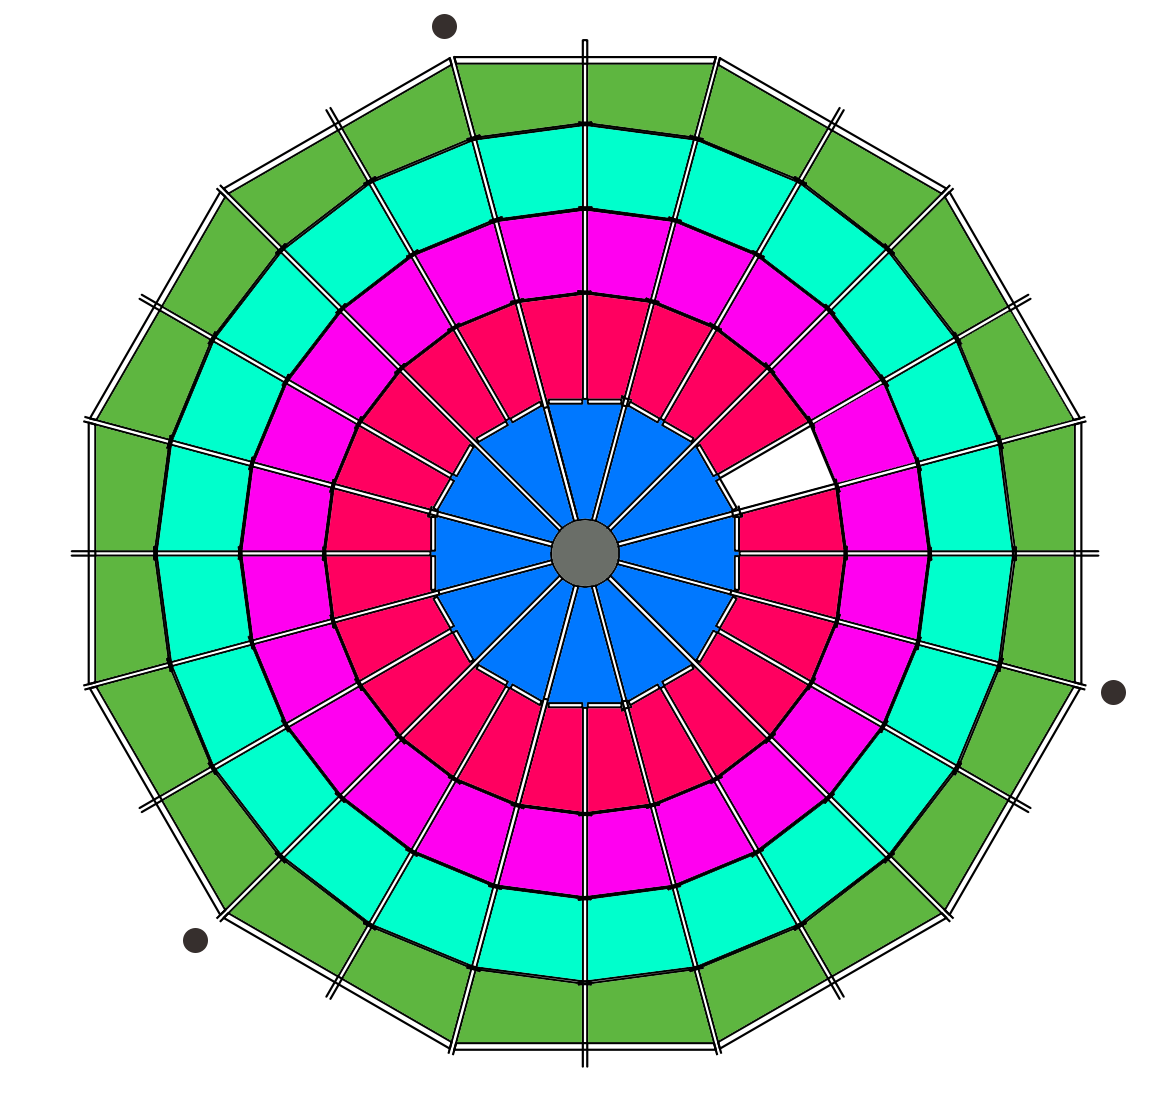
\includegraphics[width=0.5\textwidth]{antPlan.png}
\centering
\vspace{-.15in}
\caption{Panel plan.}
\label{fig:antplan}
\end{figure}

\section{Surface Spars and Bracing}
As shown in Figure \ref{fig:antplan}, the parabolic spars and associated cross bracing support the mesh.  The A-B panel overlap has a PVC cross-brace (``cross-piece''), which all holds the inner end of the intermediate support spar.  The other overlaps (B-C, C-D, D-E) have a metal strap between them. The strap is on the upper side of the PVC.  The spacing is set by the size of the mesh.

The position of the cross-piece is set by the hub and the size of panel A.  Denoting the distances as 'A' - 'E' as shown in \ref{fig:panels}, we can compute the position of the {\em far} edge of the cross-piece.  Note that the mesh follows the shape of the PVC, and the planar radial value, so it is easiest to compute the parabolic path length (denoted  by $s$, where $s=0$ at $r=0$) as opposed to the radial distance.  Radial distances may be computed numerically from the path length and vice versa.  As a shortcut here, define the mapping from radius to path-length as $f(r)$ and from path-length to radius as $f^{-1}(s)$.

Since we can mark the spar while flat on the ground as opposed to pivot along a radius, we will compute in terms of path-length $s$, but specify in terms of length along the long spars ($\sigma_L$) and the short ``intermediate'' spars ($\sigma_S$).  The offsets (shown later) are $s_{oL}$ and $s_{oS}$ respectively. That is $\sigma_{\{L,S\}}(s) = s - s_{o\{L,S\}}$. 

\subsection{Cross-Brace Spar}
The cross-brace spar is located by where panel A would end, taking the overlap in consideration.  The PVC pipe intersects the long spars on either side at an angle of 15$^o$.  The reference point on the spar is taken to be where the long side of the cross piece intersects the long spar.
\begin{figure}[H]
\includegraphics[width=1.0\textwidth]{spardims.pdf}
\centering
\vspace{-.15in}
\caption{Spar dimensions.}
\label{fig:spardims}
\end{figure}
\begin{equation}
\sigma_{A,L} = s_{AB} - s_h = \frac{A - \rho_o/2 + p/2}{\cos(15^o)} - \frac{p*\tan(15^o)}{2} - s_h
\end{equation}

The width of the cross-brace spar is
\begin{equation}
Z_{AB} = 2f^{-1}(s_{AB})\sin(15^o) - p/\cos(15^o)
\end{equation}

\subsection{Metal Strips}
The metal strips go between the long and short spars.  We've seen that the offset for the long is
\begin{equation}
s_{oL} = s_h
\end{equation}
and now we find
\begin{equation}
s_{oS} = s_{AB}*\cos(15^o) + c
\end{equation}
We find that the location of the metal strips are at
\begin{eqnarray}
s_{BC} & = & s_{AB} + (B - \rho_o)/\cos(7.5^o) \\
s_{CD} & = & s_{BC} + (C - \rho_o)/\cos(7.5^o) \\
s_{DE} & = & s_{CD} + (D - \rho_o)/\cos(7.5^o) \\
\end{eqnarray}
The spar markings can be found by subtracting $s_{oL}$ or $s_{oS}$ as appropriate.

The length of the metal strips
\begin{equation}
Z_{x} = 2f^{-1}(s_{x})\sin(7.5^o) + p/\cos(7.5^o)
\end{equation}
where $x = [BC,CD,DE]$
\end{document}
